\documentclass[10pt, oneside]{article} 
\usepackage{amsmath, amsthm, amssymb, calrsfs, wasysym, verbatim, bbm, color, graphics, geometry}
\usepackage{graphicx}
\usepackage{float}
\usepackage{longtable}
\usepackage{rotating}
\usepackage{adjustbox}
\usepackage{booktabs}
\usepackage{caption}
\usepackage[english]{babel}
\usepackage[utf8]{inputenc}
\usepackage[table]{xcolor}
\usepackage{multicol}
\usepackage{hyperref}

\geometry{tmargin=.75in, bmargin=.75in, lmargin=.75in, rmargin = .75in}  

\newcommand{\R}{\mathbb{R}}
\newcommand{\C}{\mathbb{C}}
\newcommand{\Z}{\mathbb{Z}}
\newcommand{\N}{\mathbb{N}}
\newcommand{\Q}{\mathbb{Q}}
\newcommand{\Cdot}{\boldsymbol{\cdot}}

\newtheorem{thm}{Theorem}
\newtheorem{defn}{Definition}
\newtheorem{conv}{Convention}
\newtheorem{rem}{Remark}
\newtheorem{lem}{Lemma}
\newtheorem{cor}{Corollary}


\title{Computing Infrastructure: [Course Code]}
\author{[Sofia Martellozzo]}
\date{Academic Year 2021-2022}

\begin{document}

\maketitle
\newpage
\tableofcontents

\vspace{.25in}
\newpage

\section{Computing Infrastructure}

\subsection{Introduction}
\begin{defn}
{\bf Computing Infrastructure}: Technological infrastructure that provides hardware and software for computation to other systems and services.
\end{defn}


\begin{figure}[H]
    \begin{center}
    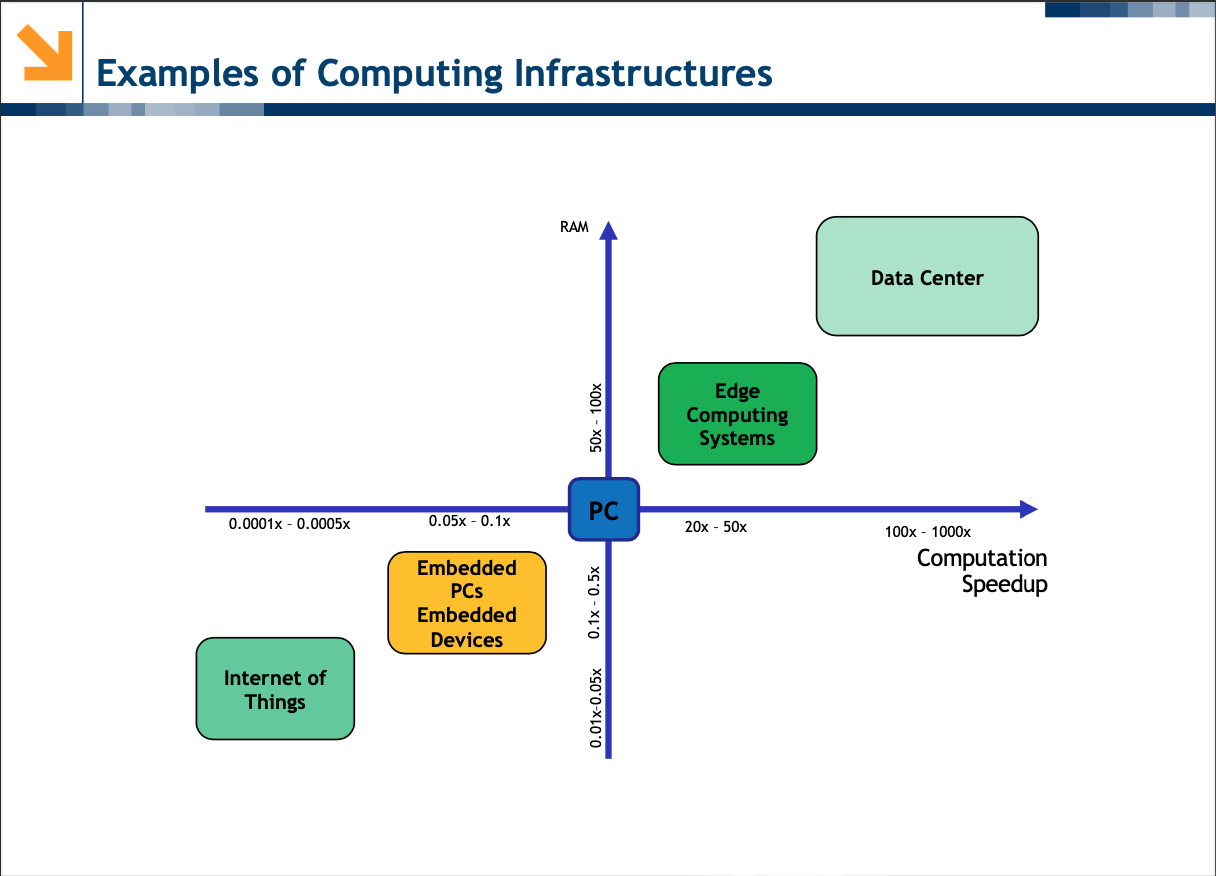
\includegraphics[width=0.5\textwidth]{img/img1.png}
    \caption{Computing Infrastructure}
    \label{fig:computing infrastructure}
    \end{center}
\end{figure}

\begin{multicols}{2}
\noindent
{\bf Advantages}:
\begin{itemize}
    \item Lower IT costs
    \item High performance
    \item Instant software updates
    \item “Unlimited” storage capacity
    \item Increased data reliability
    \item Universal document access
    \item Device Independence 
\end{itemize}

\columnbreak
\noindent
{\bf Disadvantages}:
\begin{itemize}
    \item Require a constant Internet connection
    \item Do not work well with low-speed connections
    \item Hardware Features might be limited
    \item Privacy and security issues
    \item High Power Consumption (1\% overall worldwide total energy consumption due to datacenters)
    \item Latency in making decision
\end{itemize}

\end{multicols}


\begin{figure}[H]
    \begin{center}
    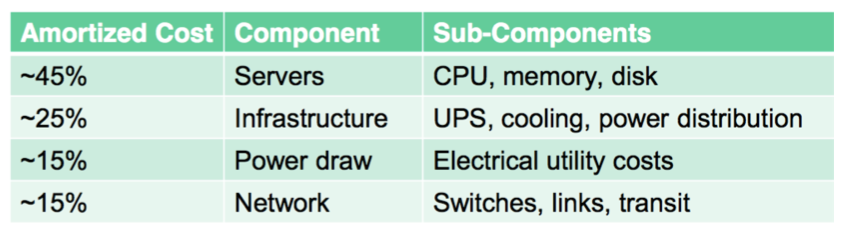
\includegraphics[width=0.5\textwidth]{img/img2.png}
    \label{fig:consumptions}
    \end{center}
\end{figure}

\newpage

%------------------------------------------------------%
\section{Data WareHouse}

\subsection{Introduction}
In the last few decades, computing and storage have moved from PC- like clients to smaller, often mobile, devices, combined with large internet services.\\
Traditional enterprises are also shifting to Cloud computing.
\begin{figure}[H]
    \begin{center}
    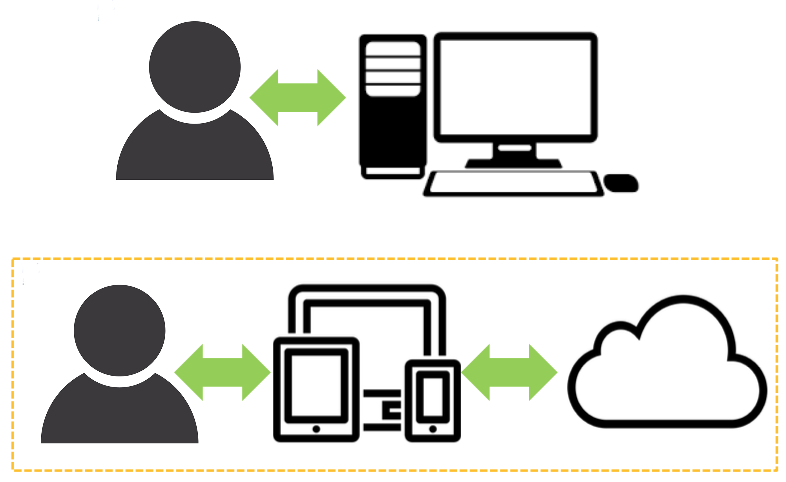
\includegraphics[width=0.5\textwidth]{img/img3.png}
    \label{fig:computing and storage}
    \end{center}
\end{figure}

\begin{multicols}{3}
\noindent
{\bf User experience improvements}
\begin{itemize}
    \item Ease of management (no configuration or backups needed)
    \item Ubiquity of access
\end{itemize}

\columnbreak
\noindent
{\bf Advantages to vendors}
\begin{itemize}
    \item Software-as-a-service allows faster application development (easier to make changes and improvements)
    \item Improvements and fixes in the software are easier inside their data centers (instead of updating many millions of clients with peculiar hardware and software configurations)
    \item The hardware deployment is restricted to a few well-tested configurations.
\end{itemize}

\columnbreak
\noindent
{\bf Server-side computing allows}
\begin{itemize}
    \item Faster introduction of new hardware devices (e.g., HW accelerators or new hardware platforms)
    \item Many application services can run at a low cost per user.
\end{itemize}

\end{multicols}
Some workloads require so much computing capability that they are a more natural fit in datacenter (and not in client-side computing).\\
A couple of examples (Search services (web, images, and so on), Machine and Deep Learning (\href{https://www.theguardian.com/commentisfree/2020/sep/08/robot-wrote-this-article-gpt-3}{GPT-3}).

\subsection{From Data Centers to Warehouse-scale computers}
{\bf Data centers} = is a place in which there are many servers\\
{\bf Whareouse} = is a type of Data Center, it works as a computer.\\
The trends toward server-side computing and widespread internet services created a new class of computing systems:
\begin{defn}
{\bf warehouse-scale computers (WSCs)}The massive scale of the software infrastructure, data repositories, and hardware platform.
\begin{itemize}
    \item is an internet service (= service provided by inyternet)
    \item may consist of tens or more individual programs (= not a single program, a collection of them that together create/provide the service)
    \item such programs interact to implement complex end-user services such as email, search, maps or machine learning.
\end{itemize}
\end{defn}
Data centers are buildings where multiple servers and communication units are co-located because of their common environmental requirements and physical security needs, and for ease of maintenance.\\
In {\bf Traditional Data Center}: typically host a large number of relatively small- or medium-sized applications, each applications is running on a dedicated hardware infrastructure that is de-coupled and protected from other systems in the same facility, applications tend not to communicate each other. Those data centers host hardware and software for multiple organizational units or even different companies.
\begin{figure}[H]
    \begin{center}
    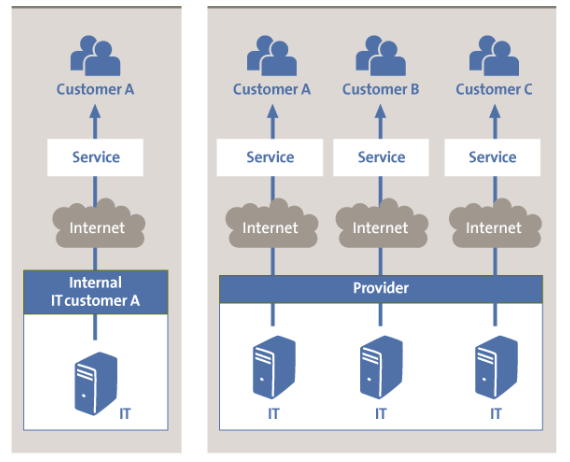
\includegraphics[width=0.3\textwidth]{img/img4.png}
    \caption{Traditional Data Center}
    \label{fig:Traditional Data Center}
    \end{center}
\end{figure}
{\bf WSCs} belong to a single organization, use a relatively homogeneous hardware and system software platform (=> easier to manage and cheaper, but has limitations on functionalities), and share a common systems management layer (such as Google, Facebook, Alibaba, Amazon, Dropbox...).\\
(you have 1 services that you want to provide to a 'huge' amount of customers)\\
Run a smaller number of very large applications (or internet services).\\
The common resource management infrastructure allows significant deployment flexibility.\\
The requirements of:
\begin{itemize}
    \item homogeneity
    \item single-organization control
    \item cost efficiency
\end{itemize}
\begin{figure}[H]
    \begin{center}
    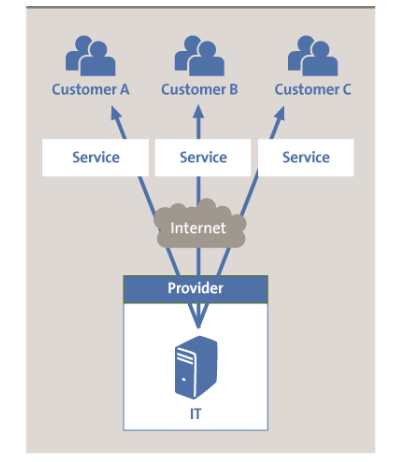
\includegraphics[width=0.25\textwidth]{img/img5.png}
    \caption{Warehouse-Scale Computers}
    \label{fig:WSCs}
    \end{center}
\end{figure}
Initially designed for online data-intensive web workloads, WSCs also now power public clouds computing systems (e.g., Amazon, Google, Microsoft). Such public clouds do run many small applications, like a traditional data center. (All of these applications rely on Virtual Machines (or Containers), and they access large, common services for block or database storage, load balancing, and so on, fitting very well with the WSC model).\\
These are not just a collection of servers: \\The software running on these systems executes on clusters of hundreds to thousands of individual servers (far beyond a single machine or a single rack)\\
+ \\The machine is itself this large cluster or aggregation of servers and needs to be considered as a single computing unit. (=$>$ scale up in terms of performance)\\
{\bf Several datacenters}:
Multiple Data Center located far apart (placed near point of iterest) => becomes important also the PRIVACY: data of a country must remain in it.\\
Multiple data centers are (often) replicas of the same service (to reduce user {\bf latency} and improve serving {\bf throughput}).\\
A request is typically fully processed within one data center.\\
{\bf Availability}:
Services provided through WSCs must guarantee high availability, typically aiming for at least 99.99\% uptime (i.e., one-hour downtime per year). Achieving such fault-free operation is difficult when a large collection of hardware and system software is involved.\\
WSC workloads must be designed to gracefully tolerate large numbers of component faults with little or no impact on service level performance and availability.

\subsection{Architectural Overview of WSCs}
Hardware implementation of WSCs might differ significantly each other; However, the architectural organization of these systems is relatively stable.
\begin{figure}[H]
    \begin{center}
    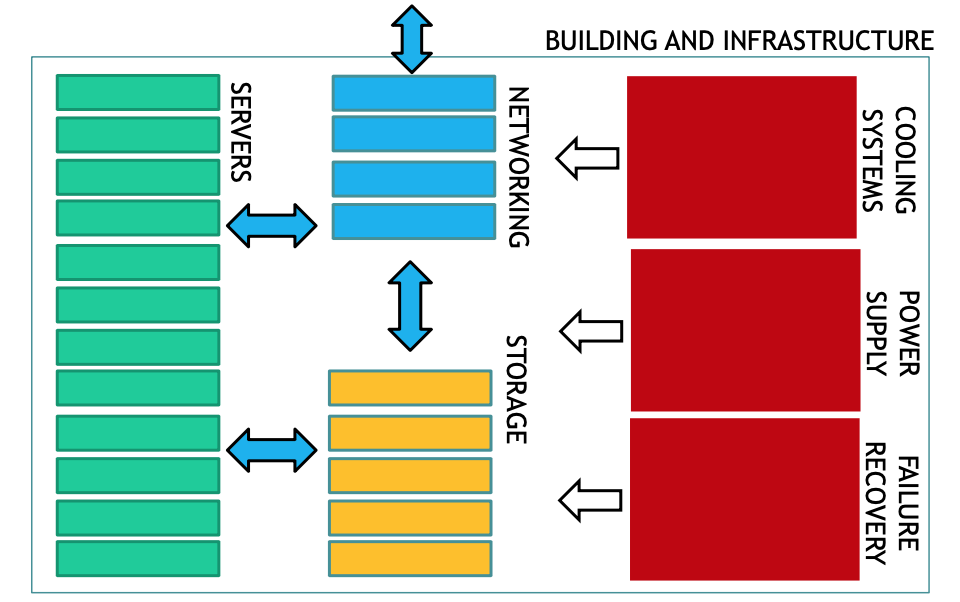
\includegraphics[width=0.4\textwidth]{img/img6.png}
    \caption{Warehouse-Scale Computers Overview}
    \label{fig:WSCs overview}
    \end{center}
\end{figure}
\begin{itemize}
    \item \color{green}\textbf{Servers}\color{black}
    : the main processing equipment
    
    \item \color{yellow}\textbf{Storage}\color{black}
    : how and where to store the information
    \begin{itemize}
        \item Disks and Flash SSDs are the building blocks of today’s WSC storage systems.
        \item These devices are connected to the data-center network and managed by sophisticated distributed systems
    \end{itemize} 
    Examples: 
    \begin{itemize}
        \item Direct Attached Storage (DAS)
        \item Network Attached Storage (NAS)
        \item Storage Area Networks (SAN)
        \item RAID controllers
    \end{itemize}
    \item \color{blue}\textbf{Networking}\color{black}
    : providing internal and external connections
    \begin{itemize}
        \item Communication equipment allows network interconnections among the devices.
    \end{itemize} 
    They can be: 
    \begin{itemize}
        \item Hubs
        \item Routers
        \item DNS or DHCP servers
        \item Load balancers
        \item Technology switches
        \item Firewalls
    \end{itemize}
    \item \color{red}\textbf{Building and Infrastructure}\color{black}
    :WSC has other important components related to power delivery, cooling, and building infrastructure that also need to be considered
\end{itemize}

%------------------------------------------------------%

\begin{figure}[H]
    \begin{center}
    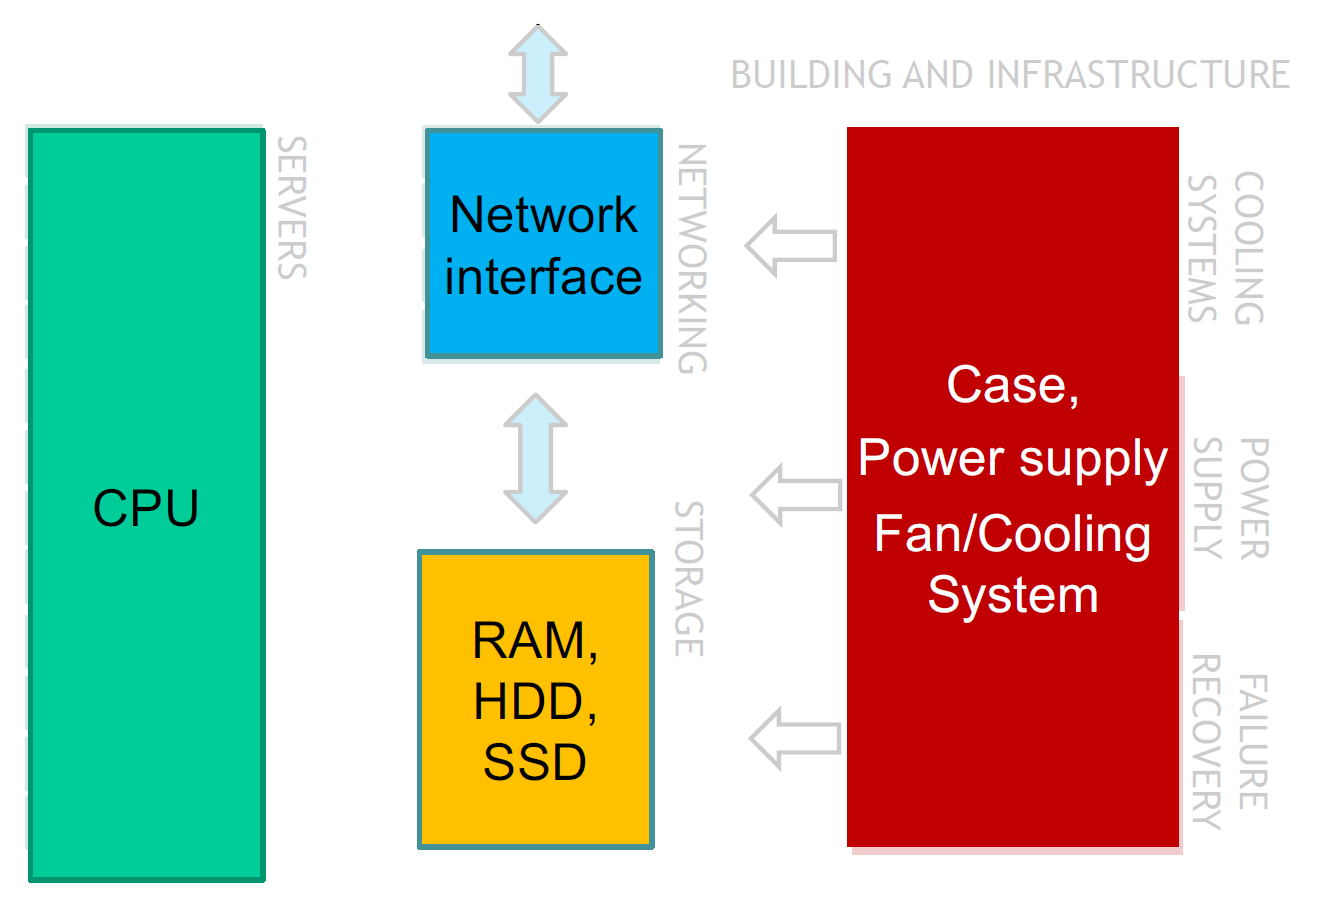
\includegraphics[width=0.4\textwidth]{img/img7.png}
    \caption{}
    \label{fig:WSCs overview2}
    \end{center}
\end{figure}
%------------------------------------------------------%
\section{Server}
\subsection{Overview}
Servers hosted in individual shelves are the basic building blocks of WSCs. They are interconnected by hierarchies of networks, and supported by the shared power and cooling infrastructure. Them are stored in the shelves (wraks) that are organized along corridors (the basic blocks of our data-center). All servers are connected to each other in the same wrak, but also (on a higher level) communicate through different wrack.
They are like ordinary PC (from a LOGISTIC point of view), but with a form factor that allows to fit them into the racks. They have 3 type of shape:
    \begin{itemize}
        \item Rack (1U or more)
        \item Blade enclosure format 
        \item Tower
    \end{itemize} 
    They may differ in: 
    \begin{itemize}
        \item Number and type of CPUs
        \item Available RAM Locally attached disks (HDD, SSD or not installed)
        \item Other special purpose devices (like GPUs, DSPs and coprocessors)
    \end{itemize}  
Servers are usually built in a tray or blade enclosure format, housing
the motherboard, chipset, additional plug-in components.

\subsubsection{The Motherboard}
The motherboard provides sockets and plug-in slots to install CPUs, memory modules (DIMMs), local storage (such as Flash SSDs or HDDs), and network interface cards (NICs) to satisfy the range of resource requirements.\\
\newline
WSCs use a relatively homogeneous hardware and
system software platform.
\newpage
\subsubsection{Chipset and additional components}
\begin{itemize}
    \item Number and type of CPUs:
\begin{itemize}
    \item From 1 to 8 CPU socket
    \item Intel Xeon Family, AMD EPYC, etc..
\end{itemize}
    \item Available RAM
    \begin{itemize}
        \item From 2 to 192 DIMM Slots
    \end{itemize}
    \item Locally attached disks:
    \begin{itemize}
        \item From 1 to 24 Drive Bays
        \item HDD or SSD (see specific lecture)
        \item SAS (higher performance but more expensive) or SATA (for entry level servers, usually cheaper)
    \end{itemize}
    \item Other special purpose devices:
    \begin{itemize}
        \item From 1 to 20 GPUs per node, or TPUs
        \item NVIDIA Pascal, Volta, etc..
    \end{itemize}
    \item Form factor:
    \begin{itemize}
        \item Form 1U to 10U
        \item Tower
    \end{itemize}
\end{itemize}
We distinguish between rack, tower and blade.\\
\newline

\subsubsection{Rack}
Racks are special shelves that accommodate all the IT equipment and allow their interconnection. The rack are used to store many {\bf Rack server}.\\ 
IT equipment must conform to specific sizes to fit into the rack shelves. Them has different hight, but same SIZE, that is {\bf standardize} (so make them easier to design): server racks are measured in rack units "U's".\\ The advantages of using these racks is that it allows designers to stack up (one on top of the others) other electronic devices along with the servers.\\
\newline
A Rack is not only a physical structure:\\
(3) The rack is the shelf that holds tens of servers together. \\(2-4) It handles shared power infrastructure, including power delivery, battery backup, and power conversion.\\
(2) There are 2 types of electronic delivery: it can provide/automatically select the server (can swich ON and OFF remotely the servers).\\
(4) It is used in case of problems with energy (power failure):
\begin{enumerate}
    \item just swich off if a power failure occur, them cannot supply all the power demand (execution)
    \item it provides 15 minutes of power, that is the time to swich on the power supply generator (source) 
\end{enumerate}
(3) The width and depth of racks vary across WSCs: some are classic 19-in wide, 48-in deep racks, while others can be wider or shallower.\\ 
(1) It is often convenient to connect the network cables at the top of the rack, such a rack-level switch is appropriately called a Top of Rack (TOR) switch.\newline\newline
\begin{figure}[H]
    \begin{center}
    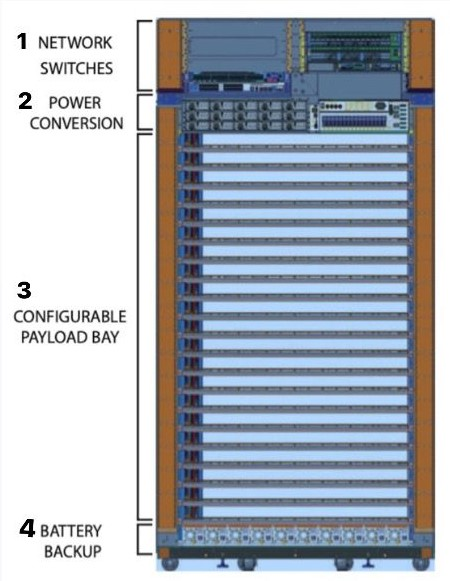
\includegraphics[width=0.4\textwidth]{img/img8.jpeg}
    \caption{RACK Servers}
    \label{fig:RACK servers}
    \end{center}
\end{figure}
Rack servers:\\
It is designed to be positioned in a bay, by vertically stacking servers one over the another along with other devices
\begin{multicols}{2}
\noindent
{\bf \color{green}Pros}\color{black}
\begin{itemize}
    \item {\bf Failure containment}: very little effort to identify, remove, and replace a malfunctioning server with another.
    \item {\bf Simplified cable management}: easy
and efficient to organize cables.
    \item {\bf Cost-effective}: Computing power and efficiency at relatively lower costs.
\end{itemize}
\columnbreak
\noindent
{\bf \color{red}Cons}\color{black}
\begin{itemize}
    \item {\bf Power usage}: Needs of additional cooling systems due to their high overall component density, thus consuming more power.
    \item {\bf Maintenance}: Since multiple devices are placed in racks together, maintaining them gets considerably tough with the increasing number of racks.
\end{itemize}
\end{multicols}



\subsubsection{Tower}
It is the simplest but is not usually adopted.
\textbf{Tower Servers}
look and feel a lot like traditional tower PCs.
Like everything they have their Pros and Cons.
\begin{multicols}{2}
\noindent
{\bf \color{green}Pros}\color{black}
\begin{itemize}
    \item {\bf Scalability and ease of upgrade}: customized and upgraded based on necessity.
    \item {\bf Cost-effective}: Tower servers are probably the cheapest of all kinds of servers
    \item {\bf Cools easily}: Since a tower server has a low overall component density, it cools down easily.
\end{itemize}
\columnbreak
\noindent
{\bf \color{red}Cons}\color{black}
\begin{itemize}
    \item {\bf Consumes a lot of space}: These servers are difficult to manage physically.
    \item {\bf Provides a basic level of performance}: a tower server is ideal for small businesses that have a limited number of clients.
    \item {\bf Complicated cable management}: devices aren't easily routed together
\end{itemize}
\end{multicols}

  
\subsubsection{Blade}
Blade servers are the latest and the most advanced type of servers in the market. They can be termed as hybrid rack servers (like orizontal rack server but placed vertically), in which servers are placed inside blade enclosures, forming a blade system. The biggest advantage of blade servers is that these servers are the smallest types of servers available at this time and are great for conserving space. A blade system also meets the IEEE standard for rack units and each rack is measured in the units of “U’s”.
\begin{multicols}{2}
\noindent
{\bf \color{green}Pros\color{black}}
\begin{itemize}
    \item {\bf Load balancing and failover}: Thanks to its much simpler and slimmer infrastructure, load balancing among the servers and failover management tends to be much simpler.
    \item {\bf Centralized management}: In a blade server, you can connect all the blades through a single interface, making the maintenance and monitoring easy.
    \item {\bf Cabling}: Blade servers don't involve the cumbersome tasks of setting up cabling. Although you still might have to deal with the cabling, it is near to negligible when compared to tower and rack servers.
    \item {\bf Size and form-factor}: They are the smallest and the most compact servers, requiring minimal physical space.
\end{itemize}
\columnbreak
\noindent
\bf{ \color{red}Cons\color{black}}
\begin{itemize}
    \item Expensive configuration: Although upgrading the blade server is easy to handle and manage, the initial configuration or the setup might require heavy efforts in complex environments.
    \item HVAC: Blade servers are very powerful and come with high component density. Therefore, special accommodations have to be arranged for these servers in order to ensure they don't get overheated. Heating, ventilation, and air conditioning systems must be managed well in the case of blade servers.
\end{itemize}
\end{multicols}

here the physical organization of a Data-Center!\\
\newline



%-------------------------------%
Deep learning models began to appear and be widely adopted, enabling specialized hardware to power a broad spectrum of machine learning solutions. To satisfy the growing compute needs for deep learning, WSCs deploy specialized accelerator hardwares:
\begin{itemize}
    \item GPU
    \item TPU
    \item FPGA
\end{itemize}
\subsubsection{Graphical Processing Units (GPU)}
\textbf{Data-parallel computations:}
the same program is executed on many data elements in parallel. The scientific codes are mapped onto the matrix operations. High level languages (such as CUDA, OpenCL, OPENACC, OPENMP, SYCL) are required. Up to 1000x faster than CPU.
\begin{figure}[H]
    \begin{center}
    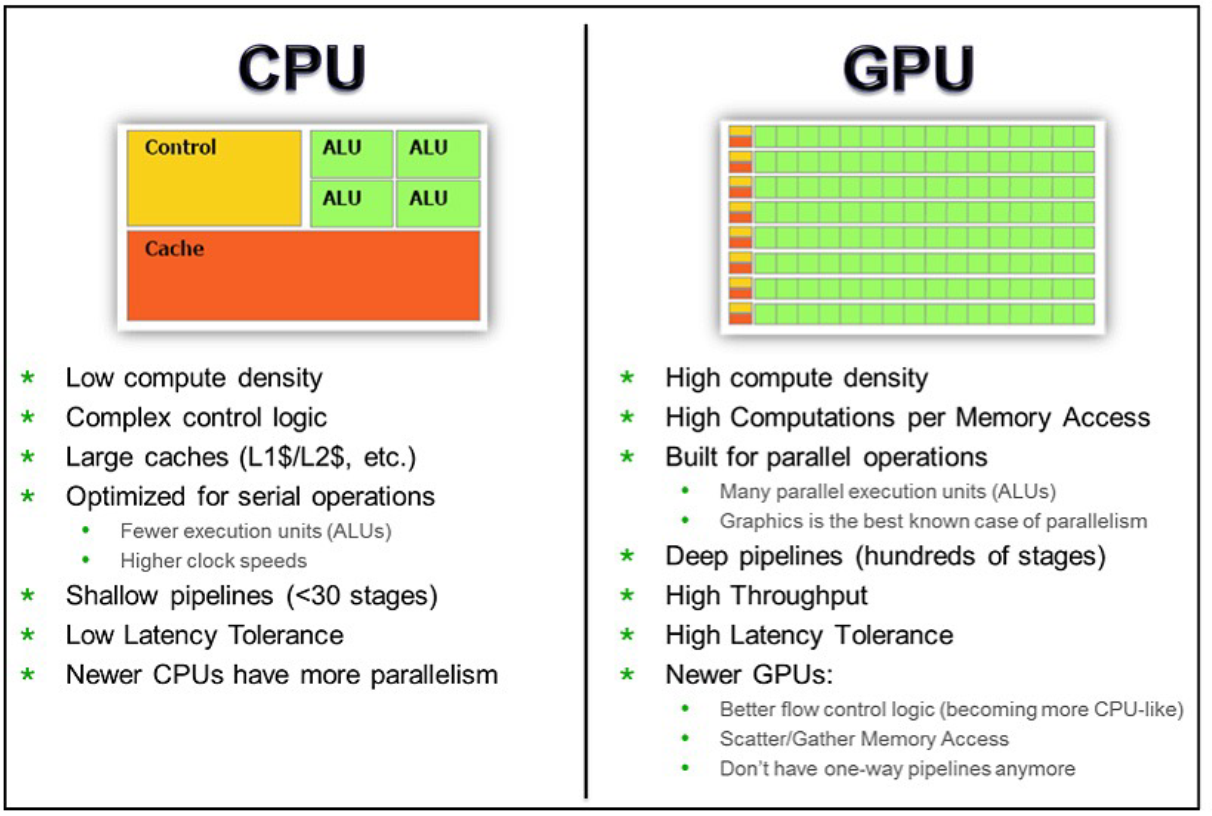
\includegraphics[width=0.4\textwidth]{img/img9.png}
    \caption{CPU vs GPU}
    \label{fig:CPU vs GPU}
    \end{center}
\end{figure}
\textbf{GPUs within the rack: PCI AND NVlink}
GPUs are configured with a CPU host connected to a PCIe-attached accelerator tray with multiple GPUs.\\GPUs within the tray are connected using high-bandwidth interconnects such as NVlink.
\textbf{NVLINK evolution and NVSwitch}
In the A100 GPU, each NVLink lane supports a data rate of 50x 4 Gbit/s in each direction. The total number of NVLink lanes increases from six lanes in the V100 GPU to 12 lanes in the A100 GPU, now yielding 600 GB/s total
\subsubsection{Tensor Processing Unit (TPU)}
While suited to ML, GPUs are still relatively general purpose devices. In recent years, designers further specialized them to ML-specific hardware Custom-built integrated circuit developed specifically for machine learning and tailored for TensorFlow.\\A Tensor is an n-dimensional matrix. This is the basic unit of operation in with TensorFlow.\\TPUs are used for training and inference:
\begin{itemize}
    \item TPUv1 is an inference-focused accelerator connected to the host CPU through PCIe links.
    \item Differently, TPUv2 and TPV3 focus training and inference
\end{itemize}
Each Tensor core has an array for matrix computations (MXU) and a connection to high bandwidth memory (HBM) to store parameters and intermediate values during computation.
\textbf{TPUv2}
\\
8 GiB of HBM for each TPU core, one MXU for each TPU core, 4 chips, 2 cores per chip.
\begin{figure}[H]
    \begin{center}
    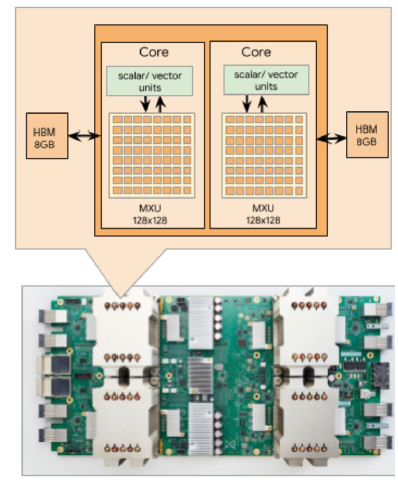
\includegraphics[width=0.4\textwidth]{img/img10.png}
    \caption{TPUv2 - 4 chips, 2 core per chip}
    \label{fig:TPUv2 - 4 chips, 2 core per chip}
    \end{center}
\end{figure}
In a rack multiple TPUv2 accelerator boards are connected through a custom high-bandwidth network to provide 11.5 petaflops of ML compute. The high bandwidth network enables fast parameter reconciliation with well-controlled tail latencies Up to 512 total TPU cores and 4 TB of total memory in a TPU Pod (64 units).
\textbf{TPUv3}
\\
TPUv3 is the first \textbf{liquid-cooled accelerator}
in Google’s data center. 2.5x faster than TPUv2. Such supercomputing-class computational power supports new ML capabilities (e.g., AutoML), and rapid neural architecture search. The v3 TPU Pod provides a maximum configuration of 256 devices for a total 2048 TPU v3 cores, 100 petaflops and 32 TB of TPU memory.
\subsubsection{Field-Programmable Gate Array (FPGA)}
Array of logic gates that can be programmed (“configured”) in the field, i.e.,by the user of the device as opposed to the people who designed it.\\ Array of carefully designed, and interconnected digital subcircuits, that efficiently implement common functions offering very high levels of flexibility. The digital subcircuits are called configurable logic blocks (CLBs).\\VHDL and Verilog are hardware description languages (HDLs), that allow to “describe” hardware. HDL code is more like a schematic that uses text to introduce components and create interconnections.\\Microsoft deployed FPGAs inside its Datacenters.
\begin{figure}[H]
    \begin{center}
    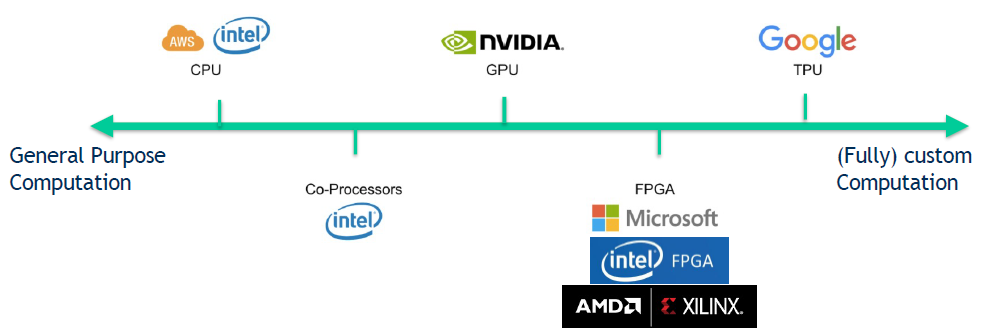
\includegraphics[width=0.4\textwidth]{img/img11.png}
    \caption{Overview}
    \label{fig:Overview}
    \end{center}
\end{figure}

\textbf{Advantages and Disadvantages}\\
\textbf{CPU Advantages:}
Easy to be programmed and support any programming framework.\\ Fast design space exploration
and run your applications.\\
\textbf{CPU Disadvantages:}
Most suited for simple AI models that do not take long to train and for small models with small training set.\\
\textbf{GPU Advantages:}
Ideal for applications in which data need to be processed in parallel like the pixels of images or videos.\\
\textbf{GPU Disadvantages:}
Programmed in languages like CUDA and OpenCL and therefore provide limited flexibility compared to CPUs.\\
\textbf{TPU Advantages:}
Very fast at performing dense vector and matrix computations and are specialized on running very fast program based on Tensorflow.\\
\textbf{TPU Disadvantages:}
For applications and models based on the TensorFlow. Lower flexibility compared to CPUs and GPUs.\\
\textbf{FPGA Advantages:}
Higher performance, lower cost and lower power consumption compared to other options like CPUs and GPU.\\
\textbf{FPGA Disadvantages:}
Programmed using OpenCL and High-level Synthesis (HLS).\\Limited flexibility compared to
other platforms.\\
\newline
\textbf{Data-center architecture}\\
The IT equipment is stored into corridors and organized into racks.
Server Racks are NEVER BACK-to-BACK. Corridors where servers are located are split into \emph{cold aisle,} 
where the front panels of the equipment is reachable, and \emph{warm aisle,}
where the back connections are located.\\ Cold air flows from the front (cool aisle), cools down the equipment, and leave the room from the back (warm aisle).


\newpage

%------------------------------------------------------%





\end{document}
